\documentclass[handout,xcolor=pdftex,dvipsnames,table]{beamer}
\usetheme{Darmstadt}
\usepackage{etex}
\providecommand\thispdfpagelabel[1]{}
\usepackage{amsmath}
\usepackage{amssymb}
\usepackage{amsthm}
\usepackage{listings}
\usepackage{graphics}
\usepackage{framed}
\usepackage{etex}
\usepackage[all]{xy}
\usepackage{svg}
\usepackage{xspace,listings,ulem,tikz}
\usepackage[outline]{contour}
\usepackage[absolute,overlay]{textpos}
\usepackage{hhline}
\usepackage[square,sort,comma,numbers]{natbib}
\usepackage{CJKutf8}
\setbeamertemplate{footline}[frame number]
\tikzset{
    onslide/.code args={<#1>#2}{% http://tex.stackexchange.com/a/6155/16595
        \only<#1>{\pgfkeysalso{#2}}
    },
    hideshow/.style args={<#1><#2>#3}{%
        onslide=<#1>{move to},
        onslide=<#2>{#3}
    }
}
\lstset{
         basicstyle=\footnotesize\ttfamily, % Standardschrift
         %numbers=left,               % Ort der Zeilennummern
         numberstyle=\tiny,          % Stil der Zeilennummern
         %stepnumber=2,               % Abstand zwischen den Zeilennummern
         numbersep=5pt,              % Abstand der Nummern zum Text
         tabsize=2,                  % Groesse von Tabs
         extendedchars=true,         %
         breaklines=true,            % Zeilen werden Umgebrochen
         keywordstyle=\color{red},
 %        keywordstyle=[1]\textbf,    % Stil der Keywords
 %        keywordstyle=[2]\textbf,    %
 %        keywordstyle=[3]\textbf,    %
 %        keywordstyle=[4]\textbf,   \sqrt{\sqrt{}} %
         %stringstyle=\color{white}\ttfamily, % Farbe der String
         showspaces=false,           % Leerzeichen anzeigen ?
         showtabs=false,             % Tabs anzeigen ?
         xleftmargin=3pt,
         framexleftmargin=3pt,
         framexrightmargin=1pt,
         framexbottommargin=3pt,
         language=C++,
         %backgroundcolor=\color{lightgray},
         showstringspaces=false      % Leerzeichen in Strings anzeigen ?        
 }

 \usetikzlibrary{arrows}
 \usepackage{caption}
\DeclareCaptionFont{white}{\color{white}}
\DeclareCaptionFormat{listing}{\colorbox[cmyk]{0.43, 0.35, 0.35,0.01}{\parbox{\textwidth}{\hspace{15pt}#1#2#3}}}
\captionsetup[lstlisting]{format=listing,labelfont=white,textfont=white, singlelinecheck=false, margin=0pt, font={bf,footnotesize}}
\beamertemplatenavigationsymbolsempty
\newcommand{\N}{\ensuremath{\mathbb{N}}} 
\newcommand{\R}{\ensuremath{\mathbb{R}}} 
\newcommand{\RR}{\ensuremath{\mathbb{R}}} 
\newcommand{\C}{\ensuremath{\mathbb{C}}} 
\newcommand{\Q}{\ensuremath{\mathbb{Q}}} 
\newcommand{\Z}{\ensuremath{\mathbb{Z}}} 
\newcommand{\D}{\ensuremath{\mathbb{D}}}
\newcommand{\lb}{\mathrm{lb}}
\newcommand{\dy}{\mathrm{dy}}
\newcommand{\cc}{\texttt{C++}\xspace}
\newcommand{\bin}{\mathrm{bin}}
\newcommand{\irram}{\texttt{iRRAM}\xspace}
\newcommand{\code}[1]{\texttt{#1}}
\newcommand{\sharpp}{\ensuremath{\#\mathcal P}\xspace}
\newcommand{\sharppu}{\ensuremath{\#{\mathcal P}_1}\xspace}
\newcommand{\fp}{\ensuremath{\mathcal{FP}}\xspace}
  \newcommand{\baana}{\code{BA\_ANA}\xspace}
  \newcommand{\anarect}{\code{ANA\_RECT}\xspace}
  \newcommand{\powerseries}{\code{POWERSERIES}\xspace}
  \newcommand{\poly}{\code{POLY}\xspace}
  \newcommand{\func}{\code{FUNC}\xspace}
  \newcommand{\real}{\code{REAL}\xspace}
  \newcommand{\complex}{\code{COMPLEX}\xspace}
	\newcommand{\abs}[1]{\left|#1\right|}
  \newcommand{\temp}{\textcolor{red}}
  \newcommand{\seq}{\mathbf}
\newcommand{\fpu}{\ensuremath{\mathcal{FP}_1}\xspace}
\DeclareMathOperator{\dom}{\mathrm{dom}}
\newtheorem{conjecture}{Conjecture} 
\newtheorem{representation1}{Representation 1} 
\newtheorem{representation1b}{Representation 1'} 
\newtheorem{representation2}{Representation 2} 
\title[data-types for multidimensional functions]{On data-types for multidimensional functions in Exact Real Arithmetic
}
\author[ H. Thies]{
		Holger Thies \footnote{Joint work with Akitoshi Kawamura and Florian Steinberg}
}
\institute[The University of Tokyo]{
  The University of Tokyo
}
\begin{document}
\setbeamercolor{note}{fg=black,bg=lightgray} 
\date{May 5, 2015}
\frame{
\titlepage
}
\section{Computing with Real Numbers}
\subsection{Computable Numbers and Functions}
\begin{frame}[t]{Outline}
 \tableofcontents 
\end{frame}
\begin{frame}
  \frametitle{Computers and Real Numbers}
  \begin{itemize}[<+->]
    \item Usually real numbers are represented by a fixed-length string (e.g. floating point)
      \item Rounding is necessary
    \item Can be implemented in hardware, thus very fast
     \item Does not behave well from a mathematical point of view (closure under composition,...) 
       \item Not a safe way to do computations
    \end{itemize}
  \end{frame}
\begin{frame}
  \frametitle{Computers and Real Numbers}
  \begin{itemize}[<+->]
  \item The set of real numbers is uncountable
    \item It is not possible to write every real number as finite string over a finite alphabet
      \item 
  \end{itemize}
  \end{frame}\begin{frame}
\frametitle{Computable Real Numbers}
  A real number is called computable if it can be approximated up to any desired precision.
  \vfill
  \pause
\begin{minipage}{.45\textwidth}
		\begin{figure}
		\centering
    \vfill
		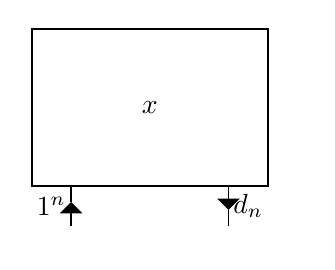
\begin{tikzpicture}<2->
				\path (0,0) rectangle (3.5,-2.7);
			%x
				\draw<2->[thick] (0,0) rectangle (3,-2);
				\node<2-> at (1.5,-1) {$x$};
				\draw<2-> (.5,-2) -- (.5,-2.2);
				\draw<2->[-triangle 90] (.5,-2.5) -- (.5,-2.2);
				\node<2-> at (.25,-2.25) {$1^n$};
				\draw<2->[-triangle 90] (2.5,-2) -- (2.5,-2.3);
				\draw<2-> (2.5,-2.3) -- (2.5,-2.5);
				\node<2-> at (2.75,-2.25) {$d_n$};
				%\node<4-> at (2.85,-2.25) {$d_{n,i}$};
				%\node<4-> at (1.5,-1) {$(a_i)$};
				%\draw<4-> (1,-2) -- (1,-2.2);
				%\draw<4->[-triangle 90] (1,-2.5) -- (1,-2.2);
				%\node<4-> at (1.25,-2.25) {$1^i$};
		\end{tikzpicture}
		\end{figure}
	\end{minipage}
	\hfill
	\begin{minipage}{.45\textwidth}
	\begin{definition}
		A real number $x$ is called computable if there is a computable function $d:\N\to\Z$, such that $ \left|\frac{d(n)}{2^{n+1}} - x\right|\leq 2^{-n}$.   
	\end{definition}
	\end{minipage}
\end{frame}
\begin{frame}
  \frametitle{Computable Functions}
	\begin{minipage}{.45\textwidth}
		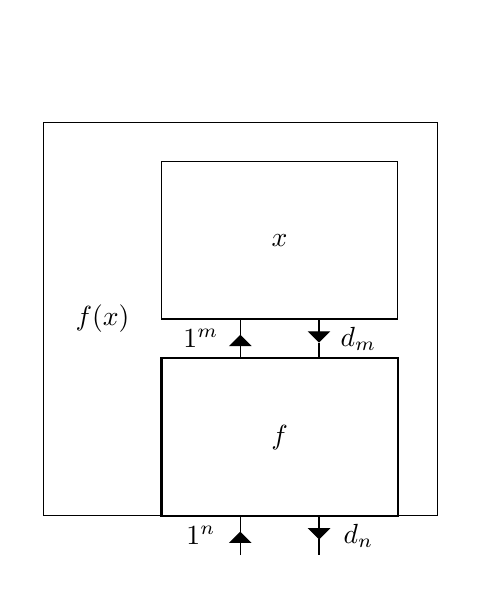
\begin{tikzpicture}
			\path (-1.7,1.7) rectangle (3.7,-5.2);
			%x
				\draw<2-> (0,0) rectangle (3,-2);
				\node<2-> at (1.5,-1) {$x$};
				\draw<2-> (1,-2) -- (1,-2.2);
				\draw<2->[-triangle 90] (1,-2.5) -- (1,-2.2);
				\node<2-> at (.5,-2.25) {$1^m$};
				\draw<2->[-triangle 90] (2,-2) -- (2,-2.3);
				\draw<2-> (2,-2.3) -- (2,-2.5);
				\node<2-> at (2.5,-2.25) {$d_m$};
			%f
				\draw<2->[thick] (0,-2.5) rectangle (3,-4.5);
				\node<2-> at (1.5,-3.5) {$f$};
				\draw<1-> (1,-4.5) -- (1,-4.7);
				\draw<1->[-triangle 90] (1,-5) -- (1,-4.7);
				\node<1-> at (.5,-4.75) {$1^n$};
				\draw<1->[-triangle 90] (2,-4.5) -- (2,-4.8);
				\draw<1-> (2,-4.8) -- (2,-5);
				\node<1-> at (2.5,-4.75) {$d_n$};
			%f(x)
				\draw<1-> (-1.5,.5) rectangle (3.5,-4.5);
				\node<1-> at (-.75,-2) {$f(x)$};
		\end{tikzpicture}
	\end{minipage}
	\hfill
	\begin{minipage}{.47\textwidth}
		\begin{definition}
			\small
			A function $f:[0,1]\to\RR$ is called computable, \newline if there is a machine that,\newline when given oracle access to approximations to the argument $x$,\newline returns approximations to the value $f(x)$.
		\end{definition}
	\end{minipage}
\end{frame}
\begin{frame}
  \frametitle{Representations}
  The definition can be generalized for general functions $f: A \to B$ with non-countable $A$ and $B$.
  
  \end{frame}
\subsection{The iRRAM framework}
\begin{frame}
  \frametitle{The \irram Framework}
  \begin{itemize}[<+->]
  \item The computational model can be implemented
  \item \irram is a \cc framework for exact real arithmetic
  \item Written by Norbert M\"{u}ller (University of Trier)
  \item \real as data type
  \item can perform arithmetic operations on \real without introducing rounding errors
  \item In the end, the user can output an approximation to the \emph{result} of the computation with any desired precision
  \item Many predefined functions already exist (sine,...)
  \item New real numbers and functions can be defined (limit operator)
  \end{itemize}
\end{frame}

\begin{frame}
  \frametitle{Complexity Theory}
  \centering
  \includegraphics[width=0.6\textwidth]{complexity}
  \end{frame}
\subsection{Analytic Functions}
\begin{frame}
\frametitle{Data-types for functions}
We want to implement a data-type for functions and perform operations on this type.
\pause
\begin{fact}
For general polynomial time computable functions, many important operators have been shown to be computationally hard.\\
For example
\pause
\begin{itemize}[<+->]
\item Polynomial time computable functions may have noncomputable derivatives. (Ko 1983)
\item Parametric maximization is NP-hard. (Ko/Friedman (1982))
\item Integration is \#P-hard. (Friedman (1984))
\end{itemize}
\end{fact}
\pause
Thus, we can not expect to have efficient algorithms for those operators unless we restrict the possible functions.
\end{frame}
\begin{frame}
\frametitle{Analytic Function}
An analytic function is a function locally given by a complex power series.\\
\begin{definition}[Analytic Function]
% \begin{columns}
% \begin{column}{0.4\linewidth}
$f : D \to \C $, $D \subseteq \C$ is analytic if for any $x_0 \in D$ the Taylor-series
$$ T(x) := \sum^\infty_{n=0} a_n(x-x_0)^n$$
converges to $f(x)$ for $x$ in a neighborhood of $x_0$.  
% \end{column}
% \begin{column}{0.4\linewidth}
% \includegraphics[width=4.5cm]{TaylorComplexConv}
% \end{column}
% \end{columns}
\end{definition}
\end{frame}
\begin{frame}
\frametitle{Some non-uniform results}

$$a_m =\frac{f^{(m)}(x_0)}{m!} 
, \,\, f(x) = \sum_{m=0}^\infty a_m(x-x_0)^k \,\ \text{ for } x \in B(x_0,R)
$$
\vfill
\begin{theorem}[Pour-El, Richards, Ko, Friedman, M\"uller (1987/1989)]
$f$ is (polytime) computable iff $(a_m)_{m \in \N}$ is.
\end{theorem}
 \onslide<2->{
From that polynomial time computability of the derivative and the anti-derivative of a function follows immediately.
}
\end{frame}
\begin{frame}
\frametitle{Some non-uniform results}
$$a_m =\frac{f^{(m)}(0)}{m!} 
, \,\, f(x) = \sum_{m=0}^\infty a_mx^k \,\ \text{ for } x \in B(0,R)
$$
\vfill
\begin{theorem}[M\"uller (1995)]
\begin{itemize}
\item The operator $f \to (a_m)_{m \in \N}$ is not computable.
\item The evaluation operator $((a_m)_{m \in \N},x) \to f(x) $ is not computable.
\end{itemize}
\end{theorem}
\pause
However, if we supply some additional (discrete) information those operators become computable.
\end{frame}
\subsection{Representing power series}
\begin{frame}
\frametitle{A practical representation for power series}
\begin{lemma}
  Let $f : [0,1] \to \R$ be real analytic.\\
  Then there exists an $l \in \N$ such that 
  $$ \forall x \in [0,1]: \, \left | \frac{f^{(j)}(x)}{j!} \right | \leq 2^l\cdot l^j $$
\end{lemma}
\pause
$l$ can be used to make a tail estimate on
$$ \left | \sum_{n \geq N} a_n z^n \right |  $$
\end{frame}
\begin{frame}[<+->]
\frametitle{Analytic Functions and Computational Complexity}
\begin{theorem}[Kawamura, R\"osnick, M\"uller, Ziegler (2013)]
  The following operators are computable in time polynomial in $n+l$, where $2^{-n}$ is the output precision.
\begin{enumerate}
\item evaluation
\item addition and multiplication
\item differentiation and anti-differentiation
\item parametric maximization
\end{enumerate}
\end{theorem}
\end{frame}
\begin{frame}
  \frametitle{Ordinary Differential Equations}
  We are further interested in the following problem:\newline
Consider Systems of Ordinary Differential Equations of the form
\begin{eqnarray*}
  \dot y_v(t) &=& F_v(t, y_1(t), \dots, y_t(t)) \\
  y_v(0) &=& 0 
\end{eqnarray*}
for $v=1,\dots,d$ and $F_v : \RR^{d+1} \to \RR$.
  \end{frame}
\begin{frame}
\frametitle{Complexity of Ordinary Differential Equations}
\begin{theorem}[Kawamura, 2010]
Consider the IVP
$$
y'(t)=f(t,y(t)) \quad;\quad y(0)=0.
$$
\pause
There exist functions $f: [0,1] \times [-1,1] \to \RR$ and $y: [0,1] \to [-1,1]$
such that $f$ is computable in polynomial time and Lipschitz continuous
but $y$ is PSPACE-hard.
\end{theorem}
The problem can be solved in PSPACE by applying the Euler method. (Ko)
\end{frame}
\begin{frame}
  \frametitle{Ordinary Differential Equations}
  We are further interested in the following problem:\newline
Consider Systems of Ordinary Differential Equations of the form
\begin{eqnarray*}
  \dot y_v(t) &=& F_v(t, y_1(t), \dots, y_t(t)) \\
  y_v(0) &=& 0 
\end{eqnarray*}
for $v=1,\dots,d$ and $F_v : \RR^{d+1} \to \RR$.
\pause
This is hard in the general case.
\pause
But if all $F_v$ are analytic, the solutions $y_v$ will again be analytic and the coefficients of the power series
can be computed in polynomial time if the $F_v$ are polynomial time computable.
  \end{frame}
\begin{frame}
  \frametitle{Multi-Dimensional Functions}
  Consider functions $f: \RR^d \to \RR$ complex analytic in a neighborhood of $0 \in \C^d$ and their power series $\sum_{n_1, \dots, n_d \in \N} a_{n_1,\dots,n_d}x_1^{ n_1 } \dots x_d^{ n_d }$
  \begin{itemize}
  \item The beforementioned representation can be generalized for the multi-dimensional case
    \item Let $B$ and $q_i$ s.t. 
$ \abs{a_{i_1, \dots, i_d}} \leq \frac{B}{q_1^{i_1} \dots q_d^{i_d}} $
    \item Let $b_{i_1} := \sum_{i_2, \dots, i_d \in \N^{d-1}} a_{i_1, \dots, i_d} \cdot x_2^{i_2} \dots x_d^{i_d}$.
    \item Then $f(x_1, \dots, x_d) = \sum_{i \in \N} b_i\cdot x^i$
\item $\abs{b_i} \leq \frac{B}{q_1^i \cdot (1-\frac{x_2}{q_1}) \dots (1-\frac{x_d}{q_d})}$
  \item $b_i$ can be computed by evaluating a $d-1$ dimensional analytic function
  \end{itemize}
  \end{frame}
\section{Implementation}
\begin{frame}
  \frametitle{DAG approach}
  \begin{center}
        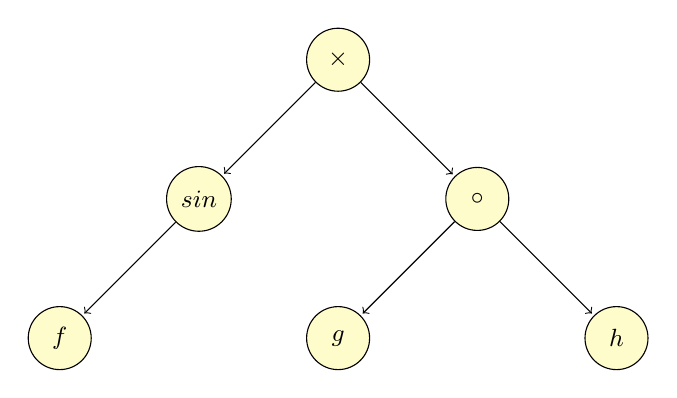
\begin{tikzpicture}[remember picture 
            ,->,shorten >=1pt,auto,node distance=2.5cm,minimum
              size=0.8cm,main node/.style={circle,fill=yellow!20,draw,font=\sffamily\small}]
    
    \node<2->[main node] (1) {$\times$};
    \node<2->[main node] (2) [below left of=1] {$sin$};
    \node<2->[main node] (6) [below left of=2] {$f$};
    \node<2->[main node] (3) [below right of=1] {$\circ$};
    \node<2->[main node] (4) [below left of=3] {$g$};
    \node<2->[main node] (5) [below right of=3] {$h$};

    \path<2->[every node/.style={font=\sffamily\small}]
    (1) edge (2)
    (2) edge (6)
    (1) edge (3)
    (3) edge (4)
    (3) edge (5);
  \end{tikzpicture}
  \end{center}
        \vfill
  Such a DAG can be evaluated or transformed to an analytic function.
\end{frame}
\begin{frame}
  \frametitle{Implementation}

  \end{frame}
\begin{frame}
  \frametitle{ODE solving}
  \end{frame}
%{
%\makeatletter % to change template
%    \setbeamertemplate{headline}[default] 
%    \def\beamer@entrycode{\vspace*{-\headheight}} 
%\makeatother
%\begin{frame}{References}
%\fontsize{6pt}{7.2}\selectfont 
%\nocite{*}
%\def\newblock{}
%\bibliographystyle{abbrv}

%\begin{thebibliography}{10}   
%
%  \beamertemplatearticlebibitems
%  \bibitem{6}
%	Harvey Friedman,
%    \newblock \emph{ The computational complexity of maximization and integration}, Adv. in Math. 53 (1984), no. 1, 80-98. MR 748898 (86c:03037)
%  \beamertemplatearticlebibitems
%  \bibitem{1}
%	Akitoshi Kawamura, Norbert Th. M\"{u}ller, Carsten R\"{o}snick, and
%Martin Ziegler
%    \newblock \emph{Parameterized Uniform Complexity in Numerics:
%from Smooth to Analytic, from NP-hard to Polytime}, pre-print (2012).
%
%  \beamertemplatearticlebibitems
%  \bibitem{7}
%	Ker-I Ko,
%    \newblock \emph{ Complexity theory of real functions}, Progress in Theoretical Computer Science, Birkh\"{a}user Boston Inc., Boston, MA, 1991.
%MR 1137517 (93i:03057)
%
%  \beamertemplatearticlebibitems
%  \bibitem{8}
%	Ker-I Ko,
%    \newblock \emph{  On the Computational Complexity of Ordinary Differential Equations}, Information and Control 58(1-3): 157-194 (1983)
%
%
%  \beamertemplatearticlebibitems
%  \bibitem{2}
%	Norbert Th. M\"{u}ller,
%    \newblock \emph{ The \irram: Exact Real Arithmetic in C++}, Computability and Complexity in Analysis (2000) .
%
%  \beamertemplatearticlebibitems
%  \bibitem{Mul95}
%	Norbert Th. M\"{u}ller,
%    \newblock \emph{ Constructive aspects of analytic functions}, Computability
%and Complexity in Analysis (Ker-I Ko and Klaus Weihrauch, eds.),
%Informatik Berichte, vol. 190, FernUniversit\"{a}t Hagen, September
%1995, CCA Workshop, Hagen, August 19-20, 1995, pp. 105-114.
%
%  \beamertemplatearticlebibitems
%  \bibitem{4}
%	Norbert Th. M\"{u}ller,
%    \newblock \emph{ Uniform Computational Complexity of Taylor Series}, ICALP 1987: 435-444
%
%  \beamertemplatearticlebibitems
%  \bibitem{5}
%	Norbert Th. M\"{u}ller,
%    \newblock \emph{ Polynomial Time Computation of Taylor Series}, Proc. 22 JAIIO - PANEL 1993
%
%  \beamertemplatearticlebibitems
%  \bibitem{9}
%	Marian B. Pour-El and J. Ian Richards,
%    \newblock \emph{ Computability in analysis
%and physics}, Perspectives in Mathematical Logic, Springer-Verlag,
%Berlin, 1989. MR 1005942 (90k:03062)
%  \beamertemplatearticlebibitems
%  \bibitem{11}
%	Florian Steinberg,
%    \newblock \emph{A type of Taylor series for the C++ library iRRAM for exact real arithmetic} (draft) last edited November 28, 2013
%  \beamertemplatearticlebibitems
%  \bibitem{10}
%	Klaus Weihrauch,
%    \newblock \emph{Computable analysis}, Texts in Theoretical Computer
%Science. An EATCS Series, Springer-Verlag, Berlin, 2000, An
%introduction. MR 1795407 (2002b:03129)
%
%  \end{thebibliography}

%\end{frame}
%}
\end{document}
